\newcommand{\YEAR}{2015}
\newcommand{\SEMESTER}{FS \YEAR}
\newcommand{\SUBTITLE}{Untertitel}
\newcommand{\DATE}{{\today}}
\newcommand{\TITLE}{Functional Kafka}
\newcommand{\AUTHOR}{Marc Juchli, Lorenz Wolf}
\newcommand{\SUPERVISOR}{Prof Dr. Josef Joller}
\newcommand{\EXPERT}{Dr. Simon Meier}
\newcommand{\EMAIL}{\{l1wolf, mjuchli\}@hsr.ch}
\newcommand{\KEYWORDS}{Bachelor Thesis, Computer Science, HSR, \SUBTITLE, \TITLE}

\documentclass[11pt,oneside,a4paper,parskip,listof=numbered]{scrreprt}
\usepackage[inner=2.5cm,outer=2cm,top=2cm,bottom=2cm,includefoot]{geometry}

\usepackage{cmbright}
\setlength{\parindent}{0pt}
\setlength{\parskip}{6pt plus 2pt minus 1pt}
\setlength{\emergencystretch}{3em}  % prevent overfull lines

\usepackage[T1]{fontenc}
\usepackage[utf8]{inputenc}
%/usepackage{ngerman}
\usepackage{graphicx}
\usepackage{color}
\usepackage{ccicons}
\usepackage{rotating}
\usepackage[colorlinks=true, linkcolor=blue, urlcolor=blue, citecolor=blue]{hyperref}
\usepackage{pdfpages}
\usepackage{todonotes}
\usepackage{tabularx}
\usepackage{xcolor,colortbl}
\usepackage{pdflscape}
\usepackage{soul}
\usepackage{glossaries}
\usepackage{amsmath}
\usepackage{amssymb}
\usepackage{pifont}
\usepackage{fourier}
\usepackage{MnSymbol}
\usepackage{wasysym}
\usepackage{float} % Bilder fix positionieren
\usepackage{appendix}
\usepackage{booktabs}
\usepackage{makeidx}
\makeindex
\usepackage{fancybox}
\usepackage[nottoc,numbib]{tocbibind}
\usepackage{enumitem}
% \usepackage{slashbox} %halbierte Tabellenzellen
% \setlist{nolistsep}
\setlist[itemize]{noitemsep, topsep=0pt}

\usepackage{tikz}
\usepackage{pgf-umlsd}
\usepgflibrary{arrows} % for pgf-umlsd

% \let\stdsection\section
% \renewcommand\section{\newpage\stdsection}

\subject{\SUBTITLE}
\title{\TITLE}
\author{\AUTHOR \\ \EMAIL}

\hypersetup{
  pdftitle    = {\TITLE},
  pdfsubject  = {\SUBTITLE},
  pdfauthor   = {\AUTHOR, \EMAIL},
  pdfkeywords = {\KEYWORDS} ,
  pdfcreator  = {pdflatex},
  pdfproducer = {LaTeX with hyperref}
}


\newcommand{\logoLX}{\fcolorbox{white}{red}{\textcolor{white}{LX}}}
\newcommand{\logoSH}{\fcolorbox{white}{maroon}{\textcolor{white}{SH}}}
\newcommand{\logoSE}{\fcolorbox{white}{orange}{\textcolor{white}{SE}}}
\newcommand{\logoXJ}{\fcolorbox{white}{darkblue}{\textcolor{white}{XJ}}}
\newcommand{\logoXC}{\fcolorbox{white}{darkgreen}{\textcolor{white}{XC}}}
\newcommand{\logoMF}{\fcolorbox{white}{lila}{\textcolor{white}{M4}}}
\newcommand{\logoMS}{\fcolorbox{white}{violett}{\textcolor{white}{M6}}}
\newcommand{\logoMN}{\fcolorbox{white}{pink}{\textcolor{white}{MN}}}

\newcommand{\verwundbar}{\hfill \fcolorbox{black}{red}{(Verwundbar \bomb)}}
\newcommand{\nichtverwundbar}{\hfill \fcolorbox{black}{green}{(Nicht verwundbar~\sun)}}
\newcommand{\zelleverwundbar}{\cellcolor{red} \bomb}
\newcommand{\zellenichtverwundbar}{\cellcolor{green} \sun}
\newcommand{\zelleteilweiseverwundbar}{\cellcolor{yellow} \danger }
\newcommand{\gegenmassnahme}{$\rightarrow$ Die Gegenmassnahme ist in diesem Kapitel zu finden: }
\newcommand{\keinegegenmassnahme}{$\rightarrow$ Diese Verwundbarkeit lässt sich mit keiner Gegenmassnahme beheben.}

\definecolor{yellow}{RGB}{240,173,78}
\definecolor{orange}{RGB}{255,128,0}
\definecolor{lila}{RGB}{128,128,192}
\definecolor{violett}{RGB}{64,0,128}
\definecolor{pink}{RGB}{255,128,192}

% Code-Listing
\definecolor{gray}{rgb}{0.4,0.4,0.4}
\definecolor{darkblue}{rgb}{0.0,0.0,0.6}
\definecolor{cyan}{rgb}{0.0,0.6,0.6}
\definecolor{green}{RGB}{92,184,92}
\definecolor{red}{RGB}{217,83,79}
%\definecolor{light-gray}{gray}{0.95}
%\definecolor{lbcolor}{rgb}{0.9,0.9,0.9}
\usepackage{listings}
\definecolor{maroon}{rgb}{0.5,0,0}
\definecolor{darkgreen}{rgb}{0,0.5,0}
\definecolor{sh_comment}{rgb}{0.12, 0.38, 0.18 } %adjusted, in Eclipse: {0.25, 0.42, 0.30 } = #3F6A4D
\definecolor{sh_keyword}{rgb}{0.37, 0.08, 0.25}  % #5F1441
\definecolor{sh_string}{rgb}{0.06, 0.10, 0.98} % #101AF9

% \lstset{numbers=left,
%     language=Java,                               % oder C++, Pascal, {[77]Fortran}, ...
%     basicstyle=\ttfamily,                        % Textgröße des Standardtexts
%     keywordstyle=\ttfamily\color{red},           % Formattierung Schlüsselwörter
%     commentstyle=\ttfamily\color{green},         % Formattierung Kommentar
%     stringstyle=\ttfamily\color{blue},           % Formattierung Strings
%     breaklines=true,                             % Umbruch langer Zeilen
%     showstringspaces=false,                      % Spezielles Zeichen für Leerzeichen
% }
\lstset {
 frame=rlbt,
 rulesepcolor=\color{black},
 showspaces=false,showtabs=false,tabsize=2,
 %numberstyle=\tiny,numbers=left,
 basicstyle=\ttfamily\footnotesize,
 stringstyle=\color{sh_string},
 keywordstyle = \color{sh_keyword}\bfseries,
 commentstyle=\color{darkgreen}\itshape,
 captionpos=b,
 %lineskip=-0.1em,
 showstringspaces=false,
 escapebegin={\lstsmallmath}, escapeend={\lstsmallmathend},
 breaklines=true, % breakatwhitespace=true,
 prebreak=\raisebox{0ex}[0ex][0ex]{\ensuremath{\rhookswarrow}},
 % postbreak=\raisebox{0ex}[0ex][0ex]{\ensuremath{\rcurvearrowse\space}}
}
\lstnewenvironment{code}{\lstset{language=Haskell}}{}

\newcommand{\inputlisting}[2][]{%
  \lstinputlisting[caption={\texttt{\detokenize{#2}}},#1]{#2}%
}

\lstdefinelanguage{XML}
{
  basicstyle=\ttfamily\footnotesize,
  morestring=[b]",
  moredelim=[s][\bfseries\color{maroon}]{<}{\ },
  moredelim=[s][\bfseries\color{maroon}]{</}{>},
  moredelim=[l][\bfseries\color{maroon}]{/>},
  moredelim=[l][\bfseries\color{maroon}]{>},
  morecomment=[s]{<?}{?>},
  morecomment=[s]{<!--}{-->},
  commentstyle=\color{darkgreen},
  stringstyle=\color{blue},
  identifierstyle=\color{red}
}

\makeglossaries
\chapter{Glossar}

\begin{description}
  \item[Artifact] Gegenstand
  \item[Socket] Communication endpoint to which an application can write data
that are to be sent out over the underlying network, and from which incoming end
data can be read. \cite{TAN06}
\end{description} 



\begin{document}
\begin{titlepage}
\begin{flushleft}

\begin{center}
\begin{minipage}[t]{0.45\textwidth}
  
\includegraphics[width=\textwidth]{images/hsr_logo.pdf}
\end{minipage}
\begin{minipage}[t]{0.45\textwidth}
 
\includegraphics[width=\textwidth]{images/haskell_kafka_logo.pdf}
\end{minipage}
\end{center}
\noindent\begin{minipage}[t]{0.49\textwidth}
  \begin{flushleft}
    \vspace{0pt} %needed else aligned to bottom
    % 
\includegraphics[width=1\textwidth]{images/hsr_logo.pdf}
  \end{flushleft}
\end{minipage}
\hfill
\begin{minipage}[t]{0.49\textwidth}
  \begin{flushright}
    \vspace{0pt} %needed else aligned to bottom
  \end{flushright}
\end{minipage}
\\[4cm]

{\huge \bfseries \TITLE}\\[2.5cm]
% {\large \bfseries \SUBTITLE}\\[2cm]

Bachelor Thesis \\
\SEMESTER \\
Computer Science Department \\
HSR - University of Applied Sciences Rapperswil \\
\url{http://www.hsr.ch/}\\[2cm]


\vfill

Authors: \AUTHOR \\
Supervisor: \SUPERVISOR \\
Expert: \EXPERT \\
Scope of work: 12 ECTS (360 hours of work per Student) \\
Duration: February 16 until June 12, 2015 \\
% Datum: {\DATE}

\end{flushleft}
\end{titlepage}

\hypersetup{linkcolor=black}
\setcounter{tocdepth}{1}
\tableofcontents

\part{Einführung}
%\begin{abstract}
 Abstract here
\end{abstract}

%\chapter{Management Summary}

\section{Introduction}

This thesis aims to adapt the concept of Apache Kafka and build a messaging
system, namely Haskell Message Broker (HMB), in the functional programming
language Haskell. Thereby the focus lies on the implementation of a stable
(related to networking) server application system as well as on the building a
log subsystem, which in Apache Kafka is considered to be the most important
feature. As Kafka comes with its own wire-protocol a part of this thesis will
focus on a fully compatible implementation of the Apache Kafka Protocol in
Haskell, including a client library allowing Haskell applications to take use of
the protocol implementation and communicate with Apache Kafka or HMB.

\section{Approach}

First of all we started to become familiar with the state of the art in
messaging, especially event streaming. As essential part of this prestudy we
analysed the approach and functionality of Apache Kafka. In this first third of
the thesis we also learned the functional paradigm and the programming language
Haskell intensively. After the prestudy phase we elaborated an architecture prototype
to demonstrate some very basic functionality of a message broker. We then
followed by working out the details for the protocol implementation and the
server application. A code review by expert Simon Meier helped us to tweak our
code and improve efficiency. Finally, we tested our system under high load to
optimize performance of our application.

\section{Results}

The first result of this thesis is the prestudy documentation, which
resumes gathered knowledge in the familiarization phase of this work.
It gives an insight in messaging fundamentals and  takes a closer look to Apache
Kafka and related topics. It can be offered for using as academic amendment for
existing lectures. Another result is the implementation of the Kafka protocol in
Haskell. The design decision of separating protocol related code from the broker
implementation leads to a isolated product which can be used as library for
different projects. The open sourced code has already been praised by the
Haskell community and found its contributors helped uncovering minor
issues. Finally, the resulting broker application provides a server
with basic functionality in networking and persisting messages. It adapts
some features of Apache Kafka and provides the ability to produce and consume
data. It supports Kafka clients as it is based on the protocol implementation
mentioned above. Simple console clients are provided to demonstrate the
functionality.

\section{Outlook}

- broker results promissing
- very extendable/scalable implementation base and architecture
- with further work one could build the current prototype to an extraordinary
broker system.

As for now, the highlight remains the protocol implementation which has already
been praised by the Haskell community and found its contributors they helped
uncovering minor issues.

\include{aufgabenstellung}


\part{Prestudy}
\chapter{Motivation} 

In distributed systems and the involved technologies, a significant amount of
terms and definitions have been given in the literature. First part of this
preparatory study aims to achieve more clarity in this confusing and oftentimes
ambiguous \textit{jungle of terminology}, whereas the focus lies on topics that
are related to Apache Kafka. After defining basic concepts for referencing
during this thesis, we go deeper into the technology and components of Apache
Kafka itself. Finally we compare other implementations of similar systems
whereas the goal of this survey is to uncover the differences of the most
related alternatives in contrast to Apache Kafka. \\

\begin{figure}[H]
    \centering
    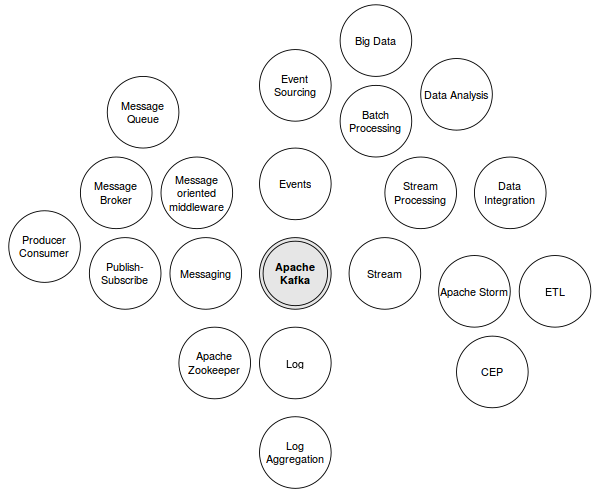
\includegraphics[width=0.6\textwidth]{images/jungle-of-terminology.png}
    \caption{\textit{Jungle of Terminology} related to Apache Kafka}
    \label{fig:jungle-of-terminology}
\end{figure}


\chapter{Introduction to Messaging} 

\section{Message Oriented Middleware}
\label{intro-messaging-mom}
Introducing an intermediate component between distributed
clients, messaging reduces the close coupling of other communication styles just
based on \gls{Socket}s or RMI. This additional component can be named as
Message-Oriented Middleware (MOM) and is all about passing \gls{Msg}s in any
format from one application to another whereas the parties do not need to know
each other directly. Thereby the main characteristic of a MOM is that its
supports a storage capacity which leads to a persistent way of communication where it is
not required that the collaborating endpoints are active during the entire
transmission of a message. This loose coupling in time is achieved by
working with queues as data structure (first-in-first-out) where applications
can insert their messages and a receiver program can read from this queue at a
different time. In normal case the original sender
never has the guarantee that the sent message has arrived at the desired
destination but it always has the confirmation of the MOM that the data has put
in a message queue. \cite{PprIBMIntro} \cite{TAN06}

\section{Interoperablity}
Because its interoperability, messaging is a very interesting communication
style for enterprise integration. Basically interoperability means that system with
different technologies can collaborate together by using the same standard or
protocols. While using a messaging system in an enterprise environment it is
much more efficient to integrate a new application to the existing data flow.
Instead of implementing a new interface for another technology, the additional
software can be just linked to the existing MOM by using the underlying
messaging protocol.\\

In the past, several companies like IBM or Microsoft developed their own
proprietary standards and protocols for asynchronous messaging systems.
Probably to keep it locked in their customer base. In June 2001 the Java Message
Service API (JMS) was released as best-known standard for messaging systems.
However, it is only an interface an not a specific protocol, JMS implementations
need to define their own. There was still no general protocol standard which
would have allowed to interoperate between different messaging implementations.
Fortunately in June 2006 a pool of multiple companies for network technologies
defined the Advanced Message Queueing Protocol (AMQP) as a open standard for an
interoperable messaging protocol. \cite{PrpAMQP}
 
%\begin{description} 
%	\item [Advanced Message Queuing Protocol (AMQP)] \hfill
%    \item [JMS]	
%\end{description}

\section{Point-To-Point Connection}
\label{intro-messaging-pointtopoint}
A Point-To-Point connection is the simplest architecture for communicating in a
messaging system. In a very basic scenario with a node A as sender of a message
and a node B as receiver, the MOM (running either on the node itself or
dedicated in the local network) assumes the task of handling a local queue for messages and manages an address-lookup
database for mapping destination names to network locations. The sender puts its
message in his local queue whereas the MOM organises the network transfer to the
queue of the target. In turn the receiver system can read from its own
local queue the incoming message. The MOM provides a specific API for both the
sender as well for the receiver:
\begin{table}[H]
\centering
\begin{tabular}{|l|l|}
\hline
\textbf{Put}    & Append a message to a specific queue                                        \\ \hline
\textbf{Get}    & Block until the specific queue is nonempty, and remove the first message    \\ \hline
\textbf{Poll}   & Check a specific queue for messages, and remove the first                   \\ \hline
\textbf{Notify} & Install a handler to be called when a message is put into a specified queue \\ \hline
\end{tabular}
\caption{Basic API for message queue implementation \cite{TAN06}}
\end{table}

This kind of communcation works well in an environment with two systems which
want to collaborate and use the advantages of messaging. But if there are more
than two nodes, the local mapping of a queue name to a foreign network location
implies that each system needs to hold the addresses of all the other nodes that it
wants to communicate with. When a target address changes, all the systems that
communicate with the target must be updated. In most scenarios there is also a need
for transforming messages in different format where these implementations have
to be made on every node, which leads to duplicating code.  For more complex
integration solutions, a centralised solution whereas the MOM runs on a location
independent platform is required. This is where the message broker comes into
game. \cite{MSDNIntegration}

\section{Message Broker}
\label{intro-messaging-broker}
A messaging system with point-to-point connections can decouple two systems
by using a managed queue on each side of a collaboration. But there is
still the need of configuration the endpoints on each party. In general, a
message broker is a dedicated component which decouples source and
target systems by assuming full responsibility for coordinating communication between
all connected nodes. Thereby the main tasks of a message broker are the
dynamically registration of endpoints, determining location of target system
(a.k.a. routing) and performing of the communication as well transformation of a
message from one format to another.\cite{MSDNIntegration} \\

\subsection{Broker Pattern}
As initial point for the detailed definition of a message broker we take the
\textit{Broker Pattern} of  \textit{Patterns of Software Architecture Volume1}
which can be used to structure distributed systems with decoupled components.
Basically it differs between two types of brokers, where the \textit{Direct
Broker} performs a initialization of a connection but the following communication
is only between the two endpoints. For messaging, the second variant
\textit{Indirect Broker}, is lot more interesting because it maintains all of
the communication between the nodes at every time. So let us define the message
broker as refinement of the Indirect Broker Pattern for message-based
communication.\cite{POSA1} 

%\subsection{Structure}
The \textit{Broker Pattern} consists of five types of participating components,
which we can adapt for a message based environment by using the common terms.

\begin{description}
    \item[Producer (adapted from Client component)] \hfill \\
        {Applications that either generating data for later processing or
        accessing a service from another client in the messaging system. In both
        cases the producer pushes its messages to the broker and in general don't care 
        about it anymore.}
    \item[Producer API (adapted from Client-Side-Proxy)] \hfill \\
        {Structural component which encapsulates messaging-specific
        functionality from the rest of the client code. Thereby, a call from the producer
        can be transformed to a message in the right format. The producer API
        directly communicates with the broker API.}
    \item[Broker] \hfill \\
        {Central component that acts as a mediator and is responsible for the
        transmission of messages from multiple producers to multiple consumers.
        A broker offers an API to the messaging clients, both for consumer and
        producer. It also must have kind of a directory for locating registered
        consumers.} 
    \item[Consumer (adapted from Server component)] \hfill \\
        {Basically the consumer is a endpoint which receives and processes a
            message for further activities. An \textit{Event-Driven-Consumer}
            handles incoming messages automatically as they are pushed from the
            broker. A \textit{Polling-Consumer} explicitly gets messages when it
            wants to receive it from the broker. If a consumer provides a
            service to other clients, it also can act as a producer for sending
            back messages as response.}
\item[Consumer API (adapted from Server-Side-Proxy)] \hfill \\
        {Structural component which encapsulates messaging-specific
        functionality from the rest of the client code. Based on incoming
        messages it calls services within the consumer component. }
\end{description}

\begin{figure}[H]
    \centering
     \begin{sequencediagram}
        %\newthread{broker}{Broker}
         \newinst[1]{producer}{Producer}
         \newinst[1]{producerProx}{Producer API}
         \newinst[1]{broker}{Broker}
        \newinst[1]{consumerProx}{Consumer API}
        \newinst[1]{consumer}{Consumer}
        \begin{messcall}
            {producer}{(1) Send Request}{producerProx}{}
        \end{messcall}
        \begin{call}
            {producerProx}{(2) Pack data}{producerProx}{}
        \end{call}
        \begin{messcall}
            {producerProx}{(3) Transmit message}{broker}{}
        \end{messcall}
        \begin{call}
            {broker}{(4) Find Consumer}{broker}{}
        \end{call}
        \begin{messcall}
            {broker}{(5) Deliver Message}{consumerProx}{} 
        \end{messcall}
        \begin{call}
            {consumerProx}{(6) Unpack Data}{consumerProx}{}
        \end{call}
        \begin{messcall}
            {consumerProx}{(7) Forward Message}{consumer}{}
        \end{messcall}
    \end{sequencediagram}
    \caption{General structure of the Broker Pattern with Event-Based
    Consumer}
    \label{fig:MB-SSD-1}
\end{figure}
%We saw that a \textit{Broker} acts like a mediator between to collaborating
%applications which do not need to know each other. The same does a message
%broker, of course in a message-oriented distributed system whereas the broker
%handles incoming messages from a source to a target and backwards.

%In such an environment it is essential that existing and new applications can be
%integrated into a single, coharent system at runtime. Often these applications
%are not speaking the same language and it need kind of a gateway for
%transforming messages into a format that can be unterstood by the receiver.
%\cite{TAN06}

%\subsection{Routing and Communicating}

%\subsection{Transformation}

\subsection{Characteristics}
As described a messaging system has its strengths in interoperability and louse
coupling of distributed computers. A message broker in turn has also many further
characteristic where we have described the most related to our work as follows:  

\begin{description}
    \item [Architecture] \hfill \\
    { A fundamental design decision for a message broker is whether consumers
    should pull data from brokers or brokers should push data to consumers. This
has direct impacts to the performance of a broker system whereas in a push-based
environment the consumers can be the bottleneck when its consumption rate falls
below the rate of production. In a pull-based system consumers which fall back
can catch up at any time whereas the risk of bottleneck lies at the broker thus
 a message broker should scale well. On the other hand in a pull-based
 environment a consumer never knows whether a message is ready for consumption
 or not. In worst case this ends up with a read loop where the consumer
 constantly need to check the queue. \cite{apachekafka} }
    \item [Delivery Reliability] \hfill \\
    {
    A reliable delivery of messages can promise a specific behaviour to producer
    and consumer. A message broker typically supports one ore more of the
    following guarantees.
    \textit{At most once} guarantees that messages may be lost but are never
    redelivered. \textit{At least once} is defined that messages are never lost
    but may be redelivered. The \textit{Exactly once} semantic which is very
    typical guarantees that each message is delivered only once. Broker system
    which use the \textit{In Order} semantic deliver messages to the consumer in
    the strict same order they are sent from the producer to the broker. 
    }
    \item [Independence] \hfill \\
    { Independence to specific technologies or systems. The more independent a
        message broker is, the better it can be integrated in a existing
        environment. The use of standards and effective standardized interfaces
        promotes independence.}
    \item [Scalability] \hfill \\
    {Ability to dynamically increase performance depending on work load.  }
    \item [Latency]\hfill \\
    {Elapsed time it takes to process a single message for consumption.  }
\item [Fault Tolerance] \hfill \\
        {Ability to recovery after a failure with minimal message loss.
        Possibility to build redundancy through clustering and replication strategy such as
        master slave\todo{gls} or state machine replication\todo{gls}. It is a significant
    characteristic how a message broker syncs its replications and decides which
    of the nodes to get active if the master fails. Also it is important that in case of
failure the system can recover as quickly as possible and with minimal
throughput deficit.   }
        \item [Persistency] \hfill \\ 
        {Ability to offer durable and persistent messages although the broker
            systems restarts, crashes or consumer is inactive for longer period of time
            (for instance batch processing system). }
    \item [Throughput] \hfill \\
        {Proportion of messages which can be sent to a broker to the amount of
        messages which can be consumed in a fixed time interval.}
\end{description}

\subsection{Publish / Subscribe Channel} 
Basically, a channel is equivalent to the managed queues we described so far. In
a channel one application can write messages and another one reads that
information from it. Because a message broker can handle multiple clients with
variable behaviour we can differ between different channel.a

Sending messages to the broker in form of publishing to a specific topic and on
the other hand receiving messages only for the specified topic, is called
publish/subscribe. In contrast to a one-to-one channel, the message broker
requires the abilities to match messages on an application based level to act as
a gateway for topic related messages. Based on the informations provided within
the messages, the broker is being able to provide the messages to the client
acting as a subscriber \cite{TAN06}. In fact, the publish/subscribe channel
delivers a copy of the topic related messages to the output channel. This also
means that there can be more than one client that consumes the topic specific
messages and thus there can be more than one subscriber. Especially this feature
of having multiple consumers of a message channel, is decisive for using a
message broker in environment where we want to process the same stream of
data in multiple ways. We will go in deeper detail to stream processing in the
following chapter. \cite{EIP03}

%\todo[inline]{Beschreibung und Sequenzdiagram: Consumer meldet sich für den
%Empfang beim Broker an } 


\chapter{Introduction to Distributed Log}
\section{What is a Distributed Log?}
- Very Simple data structure 
- append-only, totally-ordered sequence of records ordered by time (entries on
the left are older then entries on the right)
- Each entry is assigned a unique sequential log entry number. Number can be
thought as "timestamp" -> decoupling from any time system) 
- record what happend and when 
- nothing to do with "application logging", as traces an application writes
out. Application Logs are designed for human read wheras log for distributed
systems are built for programmatic accessa
- producing a persistent, re-playable record of history
\\
Origin:
- origing from databases where logs used to replicating data between databases.
Database Logs include information about records of what happend. 
- Logs as mechanism for data subscription is ideal for supporting all kings of
messaging, data flow and real-time data processing. 

Main Problem: managing distributed, concurrent changes in state.(e.g. Version
Control). Log works like version control: sequence of patches = log. When you
update you pull down just the patches an apply them to your current snapshot 

Deterministic Approach for distributed systems: 
- if you feed two deterministic pieces of code the same
input log, they will produce the same output. Applying the same log on a
replicated processes, the processes will remaining consistent across replicas. 
- Reduce the problem of making multiple machines all do the same thing to the
problem of implementing a distributed consistent log to feed these processes
input.
- State of a replica can be easy determined: describe each replica by a single
number, the timestamp for the maximum log entry it has processed. This timestamp
combined with the log uniquely captures the entire state of the replica. 

PAXOS: 
- log can be models the Problem of data consensus.  
- Paxos family of algorithm 

<`0`>
<`0`>

\chapter{Introduction to Event Streaming}

In previous chapter we defined what a message broker basically is, therefore we
can imagine how Apache Kafka works. Because Apache Kafka is build for big data
environments \todo{big data erklären} there is often mention of terms like Event or
Stream. When we want to understand what what Apache Kafka actually is for an
how it is used, we need to know what an Event Stream is.

\begin{figure}[H]
    \centering
    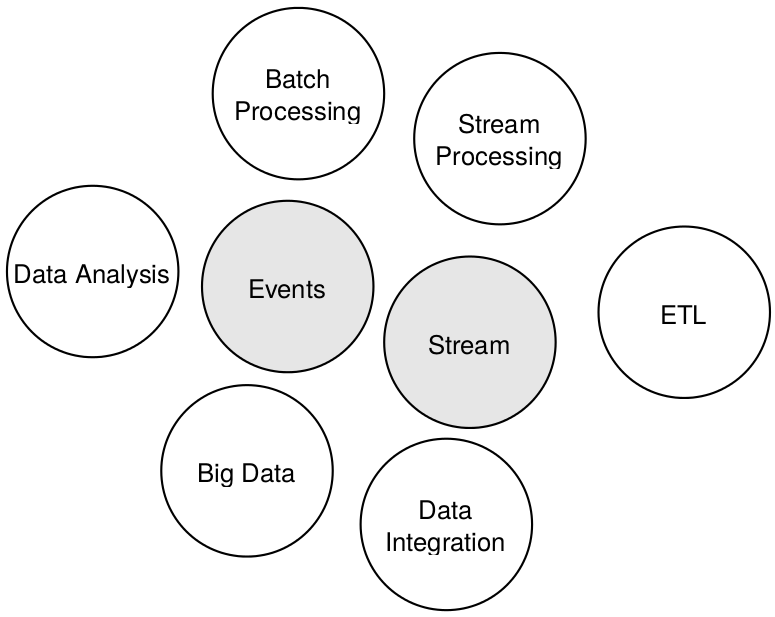
\includegraphics[width=0.45\textwidth]{images/evenstreaming-intro.png}
    \caption{Event Streaming terms}
    \label{fig:evenstreaming-intro}
\end{figure}

\section{Purpose}
The view of data as rows of databases or single files changes when one thinks
about what a business actually does with the generated data. Where retail
generates orders they lead to sales, shipments and so on, a financial
institution will generate orders they are going to have an impact of a stock
price. Or a social network platform generates clicks, impressions and searches
they are used to make some sort of intelligent analysis to further display
personalized data to it's users. Such kind of data can be thought of as streams
of events. In fact, collecting all events a business ever generated will lead to
the current state of the business and thus describe what the business did in
past. For example the current price of a stock was generated by all the orders
ever made on this stock. Every order can be captured as an event and so can all
events together reproduce the current stock price.

\section{What is an Event?}
\label{intro-datastream-datastream}
Very basically an event occurs when "something happens"  in a system like when a
user of an online shop adds an item to its basket. In modern systems, events are
transmitted as discrete messages on a MOM (see \ref{intro-messaging-mom}) and
thus following Tannenbaum et al. (2006), represent a data unit of a data
streams. Where a data stream can be applied to discrete as well as continuous
media, events are transmitted as discrete messages only. The message as itself
can be considered as an event message \cite{EIP03}.

If we think more traditionally, even database systems can be thought of as an
event based systems. The process of creating a backup in form of dumps won't
scale as we increase the frequency of dumps over time. Not only will the process
take longer according to the size of the database, also system resources are
limited during this process. An approach to make this more efficient \todo{why?}
is change capture, which describes the difference between the state of the
affected database rows before and after the change as event. If this can be done
continuously a sequence of row changes is what is being left. This in in fact,
can be described as a stream of events.

\section{Processing of Events}
Basically processing of events follows two key objectives: 
\begin{description}
    \item [Data Integration] \hfill \\ Making all the data of an organization available in all its services and systems.
    \item [Data Analytics]  \hfill \\ Preparing collected data for further analysis at any time. 
\end{description}

So data streams consisting of events as it self are not valuable but
can be taken advantage of by a system that processes these events, produces a
result and provide it to other services. This can be the calculation of the new
stock price after a customer sold his stock or the personalized content on a
news feed after a person subscribed to a new fan page. But it could also be a
more complex analysis over all the collected event that ever happened, stored in
a big database. 
\\ \\
In fact, the above mentioned examples differ in it's nature. Where the
calculation of the stock price is fairly simple by setting the price to the
latest paid stock price without any knowledge about the stock prices in past. 
In contrast, a complete analysis over a huge data base will not only require a
significant amount of processing time, it also requires some data produced in the
past. This leads to two different approaches to handle an incoming event stream
of any size: 

\begin{description}
    \item[Store raw data]  \hfill \\
    {Simply storing every single event in a big data store. Through appending
    every incoming event one get a wide history of every activity on the system.
    To analyze the data, a periodic batch process can execute big queries over
    all events to get a result.  $ \Rightarrow $  \textbf{Batch Processing}}
    \item[Store aggregated data  ] \hfill \\
    {Instead of persist every single event, directly process the incoming data stream and store
    only an aggregated summary. Because of updating the aggregation with every
    incoming event, getting an overall result is very fast (what we call
    "Real-Time"). Of course there is not a history of all the "happenings"
    anymore. $ \Rightarrow $ \textbf{Stream Processing}} 
\end{description}
\cite{TalkKleppmann}


\subsection{Batch Processing}
\label{intro-datastream-batchprocessing}
Traditional batch processing systems nowadays are distinguished between
map-reduce based and non map-reduce based systems 
\todo{cite} 

The process of  data integration (a.k.a data extraction-transformation-load, ETL
\todo{glossary}), runs at a regular time interval, such as daily, weekly or
monthly. Analyzing data that resides in a data store stage and becomes
challenging when data size grows and systems may not be able to process results
within a time limit. \cite{Liu:2014:SRP:2628194.2628251}

%\subsection{Real-time Batch Processing}
As the trend shows, the needs of performance and responsiveness in a big data
environment can't be fulfilled with traditional batch processing anymore.
Instead, real-time processing becomes more important than ever to achieve
results from queries in minutes, even seconds. 
\cite{bange2013big}

In real-time batch processing fashion, systems will address the data integration stage
with continual input of data. Processing in near-real-time [glossar] to present 
results within seconds is being addressed in data analytics. Thus,
real-time batch processing gives organization the ability to take immediate action
for those times when acting within seconds or minutes is significant.
\cite{PrpSvyOfDSPS}


\subsection{Stream Processing}
\label{intro-datastream-streamprocessing}
Stream processing refers to integration and processing of data before storing. 
A stream processing system is built out of multiple units called a processing
element (PE). Each PE receive input from their input queues, does some
computation on the input using its local state and produce output to their
output queues. PE communicate always through messaging with other PEs. 
\\ \\
Most important, those systems are optimized for high latency and high
availability. Recovering from failures is critical for a stream processing
systems and should be fast and efficient. 
Data should partitioned and handled in parallel for large volumes of data. 
The partitioning strategy of a system  affects how the system
handles the data in parallel and how the system can scale. 
\cite{PrpSvyOfDSPS}
\\ \\
Stream processing frameworks---such as Storm, Samza, or Spark
Streaming---were especially developed to provide rich processing primitives and
thus can be taken advantage of in the data integration- and processing stages.

\subsection{Other Terminology}
\subsubsection{Complex Event processing (CEP)}
In literatur there is often a confusion about the difference between
complex event processing and stream event processing. Both systems work on
events and produce results based on the properties of the events... 
- Zitat: Combines data from multiple sources  to detect patterns and attempt to
identify either opportunities or threats. The goal is to identify significant
events and respond fast. Sales leads, orders or customer service calls are
examples.\\

\todo[inline]{incomplete}

\subsubsection{Event Sourcing}
\label{event-sourcing}
Regarding to event processing we often met the term \textit{Event Sourcing} in
literature. It is a pattern originally defined by Martin Fowler which basically
treats with the same objectives as we mentioned for batch processing just with
other terms of the Domain-Driven-Design community. Instead of storing aggregated
data which represents the current state, the basic idea is to capture
every state change of an application as immutable event object. For later
analysis, this gives much richer information than just overwriting it. \todo{cite}

\section{Lambda Architecture}
While batch processing is used for data analysis to get results out of huge
amount of raw stored data at any time, stream processing reacts to events in
real time. Both approaches are very useful in different use cases. Lambda
architecture is a data-processing architecture designed to handle massive
quantities of data by taking advantage of both batch and stream processing
methods. It is split into three layers, the batch layer, the serving layer and
the speed layer:

\begin{figure}[H]
    \centering
    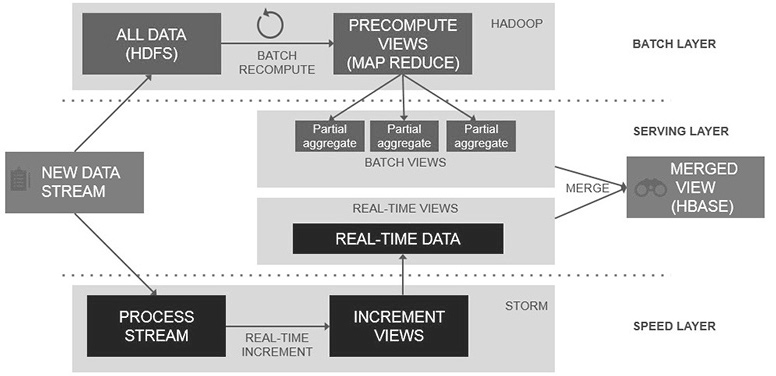
\includegraphics[width=1.0\textwidth]{images/lambda-architecture.jpg}
    \caption{Lambda Architecture}
    \label{fig:lambda-Architecture}
\end{figure}

Any query is answered through the serving layer by querying both the speed and
the batch layer. Where the badge layer periodically computes views on the
current collected data and is being outdated at the end of it's computation, the
speed layer closes this gap by constantly processing the most recent data in
near real-time fashion. \cite{marz2015big} \cite{PrpSvyOfDSPS}

\section{Centralized Event Stream}
\subsection{Need for a common data stream}
Any system which is dependent on a continuous input of data, requires a delivery
system that can provide data constantly as stream (can be
compared to an ordered message queue \todo{ref} containing events). Stream
processing systems, whether being in a lambda architecture or not, obviously
holds this requirement. On the other hand, in a big data environment there is
also the requirement of batch processing systems
(\ref{intro-datastream-batchprocessing}) being served with data. In a lambda
architecture this could be done using a stream processing framework
(\ref{intro-datastream-streamprocessing}) responsible for serving the batch
processing system with integrated data, ready for data analysis. However, an
other way of doing so would be a data store---such as the hadoop file system
(HDFS\todo{gls}---where data can be directly taken for further analysis.
The same requirement of a data store holds for any
other business intelligence system followed by the problem of the dependency of
a data store which eventually---due to the lack of an adapter---can not be
served with data by a stream processing system as comfortable as the HDFS.

\subsection{Requirements}
Facing the two types of processing events---stream- and batch
processing---together, data integration results as a common stage both system have to
deal with. Even further, for every system an organization operates, like the
data warehouse, full-text search indexes, caches or lot more, the data
integration stage will be present. 
Additionally, stream processing systems require a continuous
incoming stream to further integrate and process where batch processing systems
on the other hand demand a given persistent set of data to further integrate and analyze.

Further more, in terms of stream processing the requirement of low latency is
essential for any system of this type. For database systems combined with stream
processing, reliability becomes significantly important to handle critical updates 
such as replicating the as discussed above.
In terms of batch processing however, the demand on low latency is not as
important as the availability of well integrated data with a high throughput to
be able to handle a large volume of data in time range as low as possible.

\begin{table}[H]
\centering
\begin{tabular}{l|c|cl}
\multicolumn{1}{c|}{\textbf{}} & \textbf{Stream Processing} & \textbf{Batch
Processing} & \multicolumn{1}{c}{\textbf{}} \\ \cline{1-3}
Data Integration               & x                          & x
&                               \\
Continuous Data                & x                          &
&                               \\
Persistent Data                &                            & x
&                               \\
Low Latency                    & x                          &
&                               \\
High Throughput                     &                            & x
&
\end{tabular}
\caption{Requirements of batch and stream processing systems}
\label{table:requirements-batch-stream}
\end{table}

Note that the mentioned systems \todo{which?} do not only consume data for integration and
processing, they can also have an output. Thus, many systems are both sources and
destinations for data transfer in consequence of which a system would then need
two channels \todo{gls} per system. 
Obviously each output in this constellation is intended to be consumed by 1--N
system(s) again. Connecting all of these would lead to building a custom
channel between each pair of system (see Figure \ref{fig:datapipeline_complex}). As the set of system in an organization
rows, this would clearly become a challenge to maintain.

\begin{figure}[H]
    \centering
    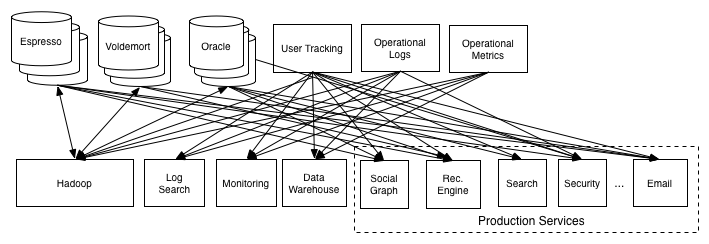
\includegraphics[width=1.0\textwidth]{images/datapipeline_complex.png}
    \caption{Complex Point-To-Point Architecture}
    \label{fig:datapipeline_complex}
\end{figure}

In this scenario several hurdles arise. The process of data integration would
have to be done for each system pair individually. At this point, an obvious
approach for a simplification would be to introduce an organization-wide
standardization of the data format. Thus, the integration process becomes 
significantly easier but still has to be done redundantly. Another problem that
remains are the tightly coupled systems. A simple change on one system could
affect one or more of it's connected systems directly, which is not only hard to
manage but also reduces the flexibility of further development of the landscape.
To extend the landscape the chances are high to touch existing systems which is
not only time intensive but also connected with risks regarding possible failures. In fact,
these are known issues of a Point-To-Point channel of traditional messaging and
is described in Section \ref{intro-messaging-pointtopoint}.

\subsection{Central Platform as Solution}
\label{intro-datastream-centralplatform}
A more elegant and reliable approach to solve the mentioned problems would be to
introduce a central platform, that is able to support both batch and real-time
consumption and thus is able to hold the described requirements given in table
\ref{table:requirements-batch-stream}. This system which can act as a single
data repository to isolated consumers and gives access to any data that is
required, as shown in figure \ref{fig:datapipeline_simple}. It aggregates
incoming events and represents an even stream for any its consumers. 

\begin{figure}[H]
    \centering
    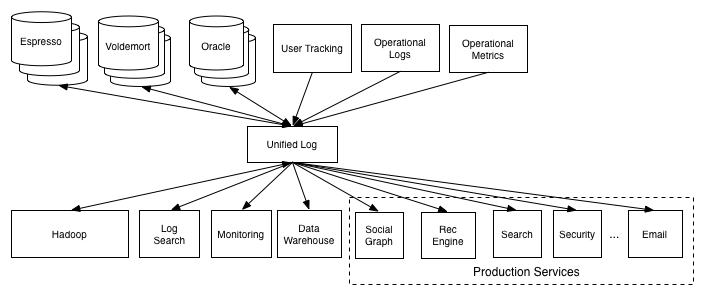
\includegraphics[width=1.0\textwidth]{images/datapipeline_simple.png}
    \caption{Broker Architecture}
    \label{fig:datapipeline_simple}
\end{figure}

In this constellation integrating a new data system---be it a data
source or a data destination---is fairly simple. Connecting it to a single
channel attached to the central platform is all what is needed to be done. Besides the
loosely coupled components, with this architecture it becomes possible to
centralize the process of data integration by doing so in a standardized way,
directly within the stream. Thus, a huge factor of complexity over the system
landscape is being reduced. In fact, this opens up a whole new set of
possibilities in organizational scalability. 

\newpage
\section{Link to Message Brokers}
As solution for a modern big data environment with huge amount of event data
which needs to be processed in different systems we need platform which acts as
mediator by handles the incoming event as stream and provide them to several
consumers (\ref{intro-datastream-centralplatform}). This seems to be very similar to
the definition of a message broker (\ref{intro-messaging-broker}) and indeed
these two concepts can be compared. Actually an event stream can be realised
with an underlying message broker and as we already described \todo{ref}, events
can be considered as messages with the event data as payload. In this point of
view the central stream platform is nothing else than a message broker which
handles incoming events, persist them in a queue and provide them for the
consumers which can be stream or batch processing systems. 
\begin{figure}[H]
    \centering
    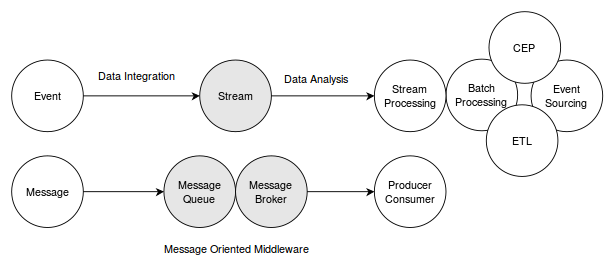
\includegraphics[width=0.8\textwidth]{images/messaging-vs-streaming.png}
    \caption{Event Stream vs Messaging}
    \label{fig:messaging-vs-streaming}
\end{figure}
Depending on the guarantees a message broker implementation provides the more it
is predestined for an event stream environment than others. In a survey (Chapter
\ref{survey-broker}) we examine the limits of traditional message brokers and
the needs for lately introduced systems such as Apache Kafka\cite{apachekafka},
Scribe\cite{scribe} or Flume\cite{apacheflume} and further try to compare and
categorize those systems after their strengths and weaknesses.

In the following Chapter \ref{intro-kafka} we examine capabilities for Apache
Kafka related to the functionalities of acting as a centralized event stream
platform. This gives not only a more concrete background of the components of a
state of the art message broker implementation but also serves as a basis for
the survey which is followed in Chapter \ref{survey-broker}.

%\section{Notes}

%-From traditional PCs and Smartphones to a lot of sensors who are connected to
%the interne -> Internet of Things!

%\todo[inline]{Einbringen des folgenden Statements: The nice thing about this
%architecture is that you can now have multiple consumers for the same event
%data. You can have one consumer which simply archives the raw events to some big
%storage; even if you don’t yet have the capability to process the raw events,
%you might as well store them, since storage is cheap and you can use them in
%future. Then you can have another consumer which does some aggregation (for
%example, incrementing counters), and another consumer which does something else.
%Those can all feed off the same event stream.}

\chapter{Survey of Message Broker implementations} 
\label{survey-broker}
In previous chapters we first discussed the traditional messaging broker as it hosts a queue
for simply move data between distributed clients without losing messages or
requiring each component to be always available. Regarding to our second topic,
the streaming of big data we defined an advanced broker with special abilities
optimized for further processing events in real-time. 

In the following survey we want to compare implementations of the most related
broker system by first defining relevant characteristics and compare the
features of each product after.

\section{Relevant Characteristics}

\section{Implementations}
%\subsection{Traditional Message Broker}

\begin{description}
    \item [Rabbit MQ] \hfill \\
    {
    Performance / Persistence:
    It is possible for persistence to underperform because the persister is
    limited in the number of file handles or async threads it has to work with.
    In both cases this can happen when you have a large number of queues which
    need to access the disk simultaneously. 
    (https://www.rabbitmq.com/persistence-conf.html)


    In a RabbitMQ Cluster, queues are
    created and live in a single node, and all nodes know about
    all the queues. When a node receives a request to a queue
    that is not available in the current node, it routes the request
    to the node that has the queue.
    To provide high availability
    (HA), RabbitMQ has a mirrored queue arranged in the
    master-slave fashion, and messages are replicated between
    master and slave, so the slave can take over if the master
    has died.
    (http://aidm.googlecode.com/svn/trunk/apache-site/research/papers/mb2.pdf)

    What RabbitMQ clustering doesn't do is provide guarantees against message loss.
    Even if you do everything right (set your messages, queues and exchanges to
    durable, etc.), when a Rabbit cluster node dies, the messages in queues on that
    node can disappear. This is because RabbitMQ doesn't replicate the contents
    of queues throughout the cluster. They live only on the node that owns the
    queue.
    (http://www.cybershovel.com/b/RabbitMQinAction.pdf
    http://pdf.th7.cn/down/files/1312/RabbitMQ%20in%20Action.pdf?yundunkey=1c4e3306d3a07226a40e927b533a8c1841426173782_179979013)

    }
    \item [Active MQ] \hfill \\
        {Note: Apache ActiveMQ is an open source message broker written in Java
    together with a full Java Message Service (JMS) client. The Replicated
    LevelDB Store uses Apache ZooKeeper to pick a master from a set of broker
    nodes configured to replicate a LevelDB Store. Then synchronizes all slave
    LevelDB Stores with the master keeps them up to date by replicating all
    updates from the master. ActiveMQ will preserve the order of messages sent
    by a single producer to all consumers on a topic. If there is a single
    consumer on a queue then the order of messages sent by a single producer
    will be preserved as well. Journal: To achieve high performance of durable
    messaging in ACtiveMQ V4.x we strongly recommend you use our high
    performance journal - which is enabled by default. This works rather like a
    database; messages (and transcation commits/rollbacks and message
    acknowledgements) are written to the journal as fast as is humanly possible
    - then at intervals we checkpoint the journal to the long term persistence
    storage (in this case JDBC).Kind of. A message can be loaded directly from the journal if it was swapped out of memory.
    The journal cannot be used, however, to recover a durable subscription as it
    does not keep an ordered index of messages per durable sub. So when a durable
    sub is activated, the journal checkpoints to flush any messages in the journal
    to the long term store and then the long term store is used to recover the
    durable subscription.Brokers cannot share a journal. Each must be
configured with it's own journal. Broker Clustering: The most common mental model of clustering in
a JMS context is that there is a collection of JMS brokers and a JMS client
will connect to one of them; then if the JMS broker goes down, it will
f we just run multiple brokers on a network and tell the clients about them
using either static discovery or dynamic discovery, then clients can easily
failover from one broker to another. However, stand alone brokers don't know
about consumers on other brokers; so if there are no consumers on a certain
broker, messages could just pile up without being consumedauto-reconnect to
another broker. } 

\end{description}


%\subsection{Streaming Broker}
\begin{description}
    \item [Apache Kafka] \hfill \\
        { (What it is) (Creator) (License) (Characteristics according features) Fault-tolerance: Beim conumse kann keine message verloren gehen da log durable, nur bei procuder kann es sein }
    \item [Amazon Kinesis] \hfill \\
    { Amazon Kinesis is a service for real-time processing of streaming big
    data. You can push data from many data producers, rapidly and continuously
as it is generated into Amazon Kinesis, which offers a reliable, highly
scalable service to capture, and store the data. ping that connects all their
distributed systems—DynamoDB, RedShift, S3, etc.—as well as the basis for
distributed stream processing using EC2. \\
 Kinesis keeps messages just for 24 hours no Log Compaction. Thus it cannot be
 used for checkpointing and state store changelogging. Another service must be
 used for durable storage.\\
    
 }
    \item [Scribe] \hfill \\
    { Push based}
    \item [Kastrell] \hfill \\
    {}
    \item [Apache Flume] \hfill \\
    {Flume is a distributed logging service specializing on being a reliable way
    of getting stream and log data into HDFS. Push based}
\end{description}

\section{Conslusion}

\todo[inline]{Welches System passt für welchen Anwendungsfall und welche nicht (Gründe)}

\chapter{Apache Kafka}
\label{intro-kafka}

As this thesis is about the implementation of a message broker that correlates
to the functionalities Apache Kafka provide, we describe in the following the
components and functionalities of Apache Kafka in the current state (Version
0.8.2). This shall provide a basis for further comparison (see \ref{survey-broker}) with
more traditional broker systems, which is why won't provide any implementation
specific details in this section but describe the concepts in a higher level of
abstractness instead. Thus, it is also an overview and the initial position of our
own implementation (see \todo{ref}), in which Chapter the implementation
specific aspects will be resolved in detail. 

\section{Background}

Apache Kafka was initially developed at LinkedIn\cite{linkedin} and subsequently
released as an open source project with the Apache Software
Foundation\cite{apachefoundation}. 
\\ \\
Initially at LinkedIn the landscape was overwhelmed by the complexity due to
point-to-point (\ref{intro-messaging-pointtopoint})
pipelines that delivered data to a single destination with no
integration between. Messages were written to aggregated files and then copied
to ETL servers (data integration) and further loaded into data warehousing and batch
processing (\ref{intro-datastream-batchprocessing})
clusters. Thus, this service included the lack of real-time data access which
is---especially for a data driven company that populates activity-driven news
feeds---an essential requirement. In fact, this fragility and complexity of this
pipeline lead to inevitable delays in adding new types of activity data.
Besides the feature wise limitations, also the detection time of operational
problems increased over time due to the ever-increasing pressure on the latency
of the data warehouse processes. This could have been solved with
stream processing systems (\ref{intro-datastream-streamprocessing}) but again, 
due to the lack of any central platform (\ref{intro-datastream-centralplatform})
that can provide continuous data, was not supported at this point.
\cite{goodhope2012building}

\\ \\
First attempts towards a piece of infrastructure (e.g. broker) that can server
stream and batch processing systems were made by experimenting with
ActiveMQ\cite{activemq}. During tests under full production load they ran into
several significant problems. It turned out that if the queue backed up beyond what could
be kept in memory, performance would severely degrade due to heavy amounts of
random I/O. Inefficiencies had to be accepted regarding clustered consumers
requiring duplicating the data for each consumer in a separate queue. Further
difficulties were faced with ActiveMQ's built in persistence mechanism that lead
to very long restart times. 
\todo[inline]{well, reasons are not that overwhelming honestly...}
According to LinkedIn it would have been possible to provide enough buffer to
keep the ActiveMQ brokers above water but would have required hundred servers to
process a subset of activity data. As a result, the decision was made to build a
custom piece of messaging infrastructure targeting high-volume scale-out
deployment and thus serve batch and stream processing systems. 
\cite{goodhope2012building}


\section{Characteristics}
- Zitat: One key feature of Kafka is its functional simplicity. While there is a
lot of sophisticated engineering under the covers, Kafka’s general functionality
is relatively straightforward. Part of this simplicity comes from its
independence from any other applications (excepting Apache ZooKeeper)

\section{Use Cases}
\begin{description}
    \item [Traditional message broker]
    \item [Log aggregation]
    \item [Stream processing] Kafka's strong durability is very useful in the
        context of stream processing
\end{description}

\section{The Log}
\label{intro-kafka-log}
Apache Kafka uses a so-called commit log for managing messages within the
broker. This log has nothing in common with "application logging", as traces of
a software designed for human read. Instead, logs in the context of distributed systems
are designed for programmatic access. Basically it is a simple, append-only data
structure which contains a sequence of records ordered by time whereas each
entry is assigned to an unique number, called offset. Thanks to the strict
ordering insight a log the record offset can be used as timestamp whereas a log
gets decoupled from any time system. \cite{apachekafka} \cite{JK-TheLog}

\begin{figure}[H]
    \centering
    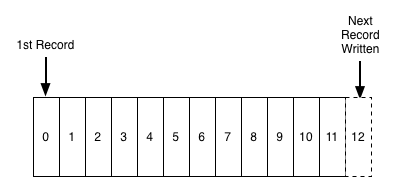
\includegraphics[width=0.4\textwidth]{images/log.png}
    \caption{The  Log \cite{JK-TheLog}}
    \label{fig:the-log}
\end{figure}

Apache Kafka handles a own log for every topic whereas the log contains all
published messages as single records. Compared to traditional messaging systems,
Kafka does not delete a record after consumption, actually it makes no difference
 whether or not they have been consumed. As we see later every consumer
controls its position of the log by its own. Instead Kafka holds record within a
defined window of data before it deletes the tail of the log. An additional
feature called log compaction can be activated to reduce the amount of messages
which need to be deleted by removing only obsolete records. \cite{apachekafka} \cite{JK-TheLog}

Facing the challenges of large distributed systems, a log must scale well. For
improving scalability and fault tolerance, Kafka can divide a log in multiple
partition. 

\begin{figure}[H]
    \centering
    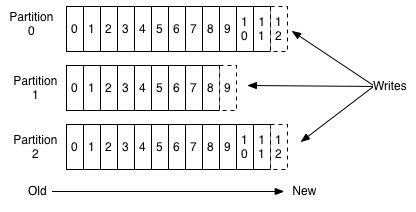
\includegraphics[width=0.5\textwidth]{images/log_anatomy.png}
    \caption{Partitioned Log \cite{apachekafka}}
    \label{fig:the-log}
\end{figure}

Logs originally come from databases where they are used to for replication
whereas the log includes records of what happened. Describing every replica by
the maximum log entry it has processed, the problem of coordinating
states of getting replicas is getting much easier. Apache Kafka uses this
approach for consumption of messages. Every consumer knows its actual offset and
advance it linearly as it reads messages from the log. The log can be seen as a
re-playable record of history whereas a consumer also can reset to an older
offset to reprocess. \cite{JK-TheLog}

\begin{figure}[H]
    \centering
    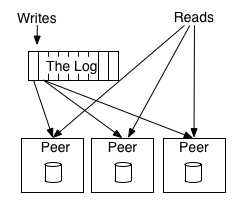
\includegraphics[width=0.4\textwidth]{images/state-machine-replication.png}
    \caption{Peers can sync their state with the log \cite{JK-TheLog}}
    \label{fig:the-log}
\end{figure}

\section{Components}
\subsection{Persistance}
Apache Kafka stores all data immediately to a persistent log
(\ref{intro-kafka-log}) 
and therefore relies heavily on the \gls{file system}.
Instead of flushing incoming messages from producers directly to the disks, the
data is stored as a compact byte structure within the \gls{page cache}.
\\ \\
The process of copying the data to the disk is handled by the operating system
that will not only use linear reads and writes \todo{gls} as a pattern for heavy
optimization but also provides read-ahead and write-behind techniques.
The latter will pre-fetch data in large block multiples and group smaller logical
writes into large physical writes. Thus, a SATA RAID-5 of six 7200rpm
disks will achieve a performance of 600MB/s in writes.
\\ \\
As a result of of the mentioned factors of using the file system and relying on
\gls{page cache} leads to the fact that Apache Kafka claims access to all free memory.
Doing so will result in a cache of up to 28-30GB on a 32GB machine. In a default
setup, data is kept in memory for 7 days to provide data required for processing
directly from the memory. This duration should be set according to of one's own
needs. In fact, the memory stays persistent during a restart of the Kafka
service but won't if the server restarts for example. In the latter scenario,
Apache Kafka will restore all data from the disk to the memory.
\\ \\
One drawback following this model of not immediately writing data to disk can not be
omitted. A small number of messages can be lost in the event of a hard server
failure before messages are transfered to the Kafka brokers or flushed to disk. 

\subsection{Message Delivery}
\label{kafka-message-delivery}
\todo[inline]{kafka = pull based model}
\todo[inline]{kafa's guarantees regarding message delivery}
\subsection{Replication}
To hold the defined guarantees (\ref{kafka-message-delivery}) regarding to system
or network failures, Apache Kafka supports \gls{replication} on the level of log
partitions \todo{ref}. Thereby it can replicate specific topics across a configurable
number of other other Kafka nodes. Every topic has a defined leader node which
is active in normal operation. A leader node can have zero or more followers
which are responsible for replicating the entries of the leader log. The followers
do this by simply act as a normal Kafka consumer of the leader node and
constantly update their own log so that it is identical. Every incoming message
needs to be replicated by every follower node before any other consumer can get
it. A fully replicated message is considered as "commited". This guarantees that
the consumer need not worry about potentially seeing a message that could be
lost if the leader fails. \cite{apachekafka}

\todo[inline]{illustration}


\todo[inline]{zookeeper}

\subsection{Compression}

\subsection{Batching}

%\subsection{The Producer}

%\subsection{The Consumer}
%While many brokered message queue systems have the broker maintain the state of
%its consumers, Kafka does not.

\subsubsection{Grouping}

\subsubsection{Ordering (offset)}

\section{Configuration Management (Zookeeper)}
\subsection{PAXO Algorithm}


\part{Technical report}

\part{Anhang}
\begin{appendices}

% Für eprints auskommentieren <<<
% \chapter{Erklärung zur Urheberschaft}

Die vorliegende Arbeit basiert auf Ideen, Arbeitsleistungen, Hilfestellungen
und Beiträgen gemäss folgender Aufstellung:

\begin{tabular}[l]{| p{8cm} | l | l |}
\hline
\textbf{Gegenstand, Leistung} & \textbf{Person} & \textbf{Funktion} \\ \hline \hline
\begin{itemize}
  \item \ldots
\end{itemize}
  & Emanuel Duss
  & Autor der Arbeit \\ \hline
\begin{itemize}
  \item \ldots
\end{itemize}
  & Roland Bischofberger
  & Autor der Arbeit \\ \hline
\begin{itemize}
  \item \ldots
\end{itemize}
  & Cyrill Brunschwiler
  & Betreuer, Industriepartner \\ \hline
\end{tabular}

Die hier nicht explizit erwähnten Teile wurden zusammen erarbeitet.

Ich erkläre hiermit,

\begin{itemize}
  \item dass ich die vorliegende Arbeit gemäss obiger Zusammenstellung selber
    und ohne weitere fremde Hilfe durchgeführt habe,
  \item dass ich sämtliche verwendeten Quellen erwähnt und gemäss gängigen
    wissenschaftlichen Zitierregeln korrekt angegeben habe,
  \item dass in der Arbeit verwendete urheberrechtlich geschützte (Copyright)
    Inhalte (insbesondere Fotografien und Grafiken) klar gekennzeichnet und mit
    Quellenhinweis versehen sind,
  \item dass Inhalte die unter Creative-Commons-Lizenz veröffentlicht wurden,
    klar gekennzeichnet sind.
\end{itemize} 

% \begin{figure}[H]
%   \centering
%   \includegraphics[width=15cm]{images/urheberschaft_unterschrift.png}
% \end{figure}

% \include{vereinbarung_weiterentwicklung}
\chapter{Projectmanagement}

\section{Introduction}

\subsubsection*{Purpose of this document}
This chapter shows the project plan for the bachelor thesis "Functional Kafka".
It is used as basis for the planning during the work. 

\subsubsection*{Goal of the project}
Analyzing Apache Kafka, a state of the art message broker system created at
LinkedIn and adapt basic features to build an alternative broker system in
Haskell. 

\section{Organization}

\subsubsection*{Structure}

\begin{tabular}[t]{|l|l|l|} \hline
\textbf{Name} & \textbf{E-mail} & \textbf{Responsibility} \\ \hline
Marc Juchli & mjuchli@hsr.ch & Research, Development, Documentation \\ \hline
Lorenz Wolf & l1wolf@hsr.ch & Research, Development, Documentation \\ \hline 
\end{tabular}

\subsubsection*{Externe Schnittstellen}

\begin{tabular}[t]{|l|l|l|} \hline
\textbf{Name} & \textbf{E-Mail} & \textbf{Responsibility}  \\ \hline
Prof Dr. Josef Joller & jjoller@hsr.ch & Supervisor \\ \hline 
Dr. Simon Meier & simon.y.meier@gmail.com & Expert  \\ \hline\end{tabular}

%\subsubsection*{Sitzungen}

%\begin{itemize}
%\item 
%\end{itemize}
\newpage
\section{Planning}
We separated the work in three phases inception, elaboration and construction
(adapted from Rational Unified Process, RUP). For planning the time schedule we
first defined tasks very rough granular. For each of those we then planed
subtasks which can be seen as single issues (see \ref{subsec:tasks}).
Furthermore three milestones were set to define particular objectives we want to
achieve at a specific time (see table \ref{tab:MeilensteineZiele}).  After reaching the
planed end of a milestone, a set-actual comparison is made (see
\ref{sec:status-tracking}). Performed work is
tracked via an Atlassian JIRA platform where we manage tasks for the project. 


\subsection{Time schedule}
\begin{figure}[H]
    \centering
    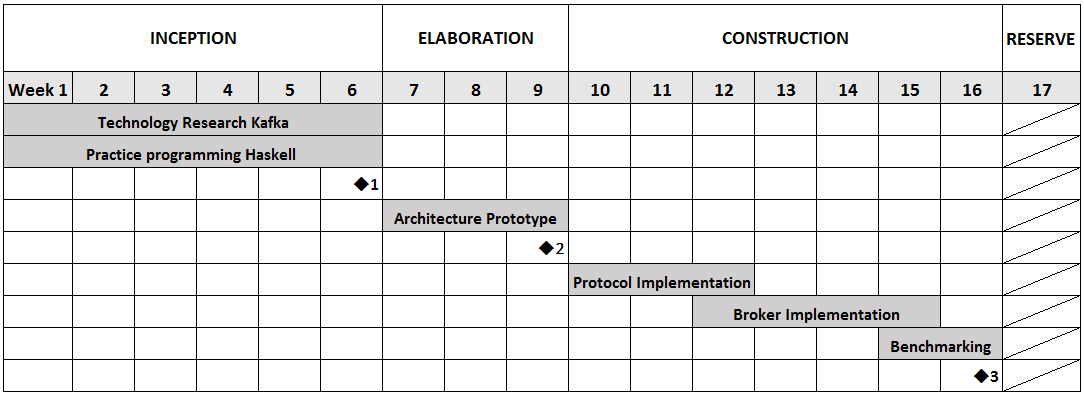
\includegraphics[width=1\textwidth]{images/workschedule.png}
    \caption{Time schedule, GANTT style}
    \label{fig:workschedule}
\end{figure}

\subsection{Milestones}
\begin{tabular}[H]{|p{4cm}|l|p{4.5cm}|p{4.5cm}|}\hline
    \textbf{Milestone} & \textbf{Deadline} & \textbf{Objectives} & \textbf{Deliverables} \\ \hline
    M0 Start of work & 16.02.2015 & - & -\\ \hline
    M1 Completion of research  & 22.03.2015 & 
        Necessary background knowledge about Kafka related topics as well as
        Haskell skills are ready for implementation part. 
        &
        Documentation technology research \\ \hline
    M2 End of elaboration & 19.04.2015 & 
        After a period of three weeks we want to have a concept and first running
        code to show some basic functionality and feasibility. 
        &
        Architecture prototype \\ \hline
    M3 End of construction & 07.06.2015 & 
        Code freeze, all planned features are implemented. Broker runs stable and
        benchmark results exist. 
        &
        Stable broker and protocol implementation. Benchmarks results. \\ \hline
  %\begin{itemize}
  %  \item \ldot
  %\end{itemize} \\ \hline
\end{tabular}
\captionof{table}{Milestones and their objectives}
\label{tab:MeilensteineZiele}

\newpage
\subsection{Tasks}
\label{subsec:tasks}
\subsubsection{Inception}


\begin{tabular}[H]{|p{6cm}|p{10cm}|}\hline
    \textbf{Task} & \textbf{Subtasks} \\ \hline
    Technology Research Kafka & 
        \begin{itemize}
            \item Learn Messaging and Event Streaming fundamentals.
            \item Analyse Apache Kafka and related topics. 
            \item Write research documentation.
        \end{itemize} \\ \hline
    Practice programming Haskell & 
        \begin{itemize}
            \item Familiarize with the functional paradigm.
            \item Setup developer environment and repositories. 
            \item Learn Haskell as functional programming language.
            \item Become acquainted to libraries regarding networking,
              building server application, and serialization.
        \end{itemize} \\ \hline
\end{tabular}
\captionof{table}{Tasks of inception phase}

\subsubsection{Elaboration}
\begin{tabular}[H]{|p{6cm}|p{10cm}|}\hline
   \textbf{Task} & \textbf{Subtasks} \\ \hline
    Architecture Prototype &
        \begin{itemize}
            \item Set up basic server architecture.
            \item Set up concept for implementing the wire protocol.
            \item Implement basic message workflow from producing messages and
            persisting at broker to consuming the data from another clients.
            \item Implement simplified clients to demonstrate architecture
                prototype prototype.
        \end{itemize} \\ \hline
   \end{tabular}
\captionof{table}{Tasks of elaboration phase}

\subsubsection{Construction}
\begin{tabular}[H]{|p{6cm}|p{10cm}|}\hline
   \textbf{Task} & \textbf{Subtasks} \\ \hline
    Protocol Implementation &
        \begin{itemize}
            \item Build standalone package providing an independent Kafka
                protocol library.
            \item Work out details of protocol implementation. Finish
                implementation of relevant parts for producing and consuming
                messages. 
            \item Implement client API for exposing simplified access to protocol
                implementation.
            \item Test Kafka compatibility.
        \end{itemize} \\ \hline
    Broker Implementation &
        \begin{itemize}
            \item Work out server application handling multiple connections
            sending produce or consume requests.
            \item Develop message log persistency adapt from Apache Kafka. 
            \item Optimize performance to approximate performance approach of
            Apache Kafka. 
        \end{itemize} \\ \hline
    Benchmarking &
        \begin{itemize}
            \item Test resulting broker implementation for performance.
            \item Comparing performance with Apache Kafka.
        \end{itemize} \\ \hline
\end{tabular}
\captionof{table}{Tasks of construction phase}

Last week of the schedule is reserved for completion work and documentation. 


\newpage
\section{Risk management}

In the table \ref{tab:Risiken} are the risk which could influence our thesis: 

\begin{tabular}[t]{|p{3cm}|p{3cm}|r|r|r|p{3cm}|p{3cm}|}\hline
\textbf{Risk} &
    \textbf{Impact} &
  \begin{sideways} \textbf{Probability } \end{sideways} &
  \begin{sideways}\textbf{Loss} \end{sideways} &
  \begin{sideways}\textbf{Risk} \end{sideways} &
  \textbf{Prevention} & \textbf{Consequences} \\ \hline
    Missing know-how in new technology & 
    Slow progress, inefficiency & 
    0.9 & 
    0.1 & 
    0.3 & 
    Ask experts before spending to much time & 
    It is part of this thesis to learn new technologies, we expect decelerated
    progress from time to time but we can deal with it. \\ \hline
  Technical impossibility & 
    No resulting product, change to other technology, loss in time. & 
    0.1 & 
    0.9 & 
    0.1 & 
    Analyse possibilities before spending to much time . &
    Inform supervisor or expert.
    \\ \hline
\end{tabular}
\captionof{table}{Risks}
\label{tab:Risiken}

%Sollte trotz den vorbeugenden Massnahmen ein zeitlicher Schaden
%entstehen, muss die Projektplanung unter Umständen angepasst werden.
%Die Zeiterfassung wird von den Projektmitarbeitern in Redmine erfasst.
%Redmine ist über folgenden Link erreichbar:
%\url{http://152.96.56.42/redmine/}. Die Projektmitarbeiter haben einen
%persönlichen Zugang  um die Daten zu erfassen. Der Betreuer hat
%ebenfalls ein Zugang, mit welchem er die Fortschritte mitverfolgen kann.
%Auf Redmine ist der aktuelle Stand des Projekts zu sehen.


%\section{Qualitätsmanagement}

%Um die Arbeitsergebnisse qualitativ auf einem hohen Niveau zu halten,
%arbeiten die Projektmitglieder nach dem Vier-Augen-Prinzip. Ein Dokument
%wird immer von beiden durchgelesen. Allfällige Änderungen werden gleich
%bilateral diskutiert und allenfalls angebracht. Somit soll erreicht
%werden, dass beide Projektmitglieder mit den Ergebnissen einverstanden
%und zufrieden sind.  Um Programmieraufgaben durchzuführen, kann
%teilweise der Ansatz von Pairprogramming eingesetzt werden. Dies führt
%dazu, dass sich beide mit dem Code auskennen.

\section{Status Tracking}
\label{sec:status-tracking}

\subsection{Milestone 1}
Milestone one was reached at 22.03.2015 by finishing the technology research
phase of our thesis. We delivered the resulting documentation, where we discuss
Messaging, Event Streaming and Apache Kafka as reference system. Originally we
had the idea to make a detailed survey about alternatives to Apache Kafka by
trying to compare them. After intensively analyzing different systems we
realized that it need much more time to give well-founded statements. Because we
wanted to comply the project plan an we had not much time anymore, we decided to
cut this part of the research documentation. This past six weeks were very
intensive not at least because we also spent a lot time in learning Haskell,
especially we had a look at topic related libraries. So we can say that our
objectives for the first milestone are achieved.

\subsection{Milestone 2}
Milestone two was reached at 19.04.2015 by finishing the architecture prototype.
Together with our supervisor we initially defined a basic workflow of publishing
messages to a server application. This workflow defined the conditions and
requirements for the architecture prototype. First we were not sure if the
planed time of only three weeks is enough to finish a runnable application. Due
to our extensive prestudy work we already had a concept in our head which we
started to implement. Actually we were very satisfied with our efficiency during
this phase. After three weeks we had a running architecture prototype which even
shows producing and consuming some date from a basic broker application. We
definitely achieved the goals of milestone two in time. 

\subsection{Milestone 3} 
Milestone three was reached at 07.06.2015 by ending the
development on broker and protocol implementation. With a duration of seven
weeks, this milestone covers the longest period of time. Because it was our
first time developing with Haskell we had many unforseen difficulties and it was
hard to estimate the cost of the tasks in this phase. In the end we spent the
most time for building a reasonable server application and to complete the
provided API's for producing and consuming messages with underlying Kafka
protocol. Also a minor issue was the implementation of a log structured
persistency on the broker. Finally we have a running prototype of a Haskell
Message Broker. But obviously there are many features remaining open, which were
not in the scope of this thesis. 

\section{Time evaluation}

\subsection{Projektstunden pro Woche}

\subsection{Projektstunden aufsummiert}

\subsection{Projektstunden pro Projektmitglied}

\subsection{Stunden pro Tätigkeitsbereich}

% \chapter{Persönliche Berichte}

\section{Bericht: Marc Juchli}

\subsection{Aufgabenstellung}
\subsection{Teamarbeit}
\subsection{Negative Erfahrungen}
\subsection{Positive Erfahrungen}


\section{Bericht: Lorenz Wolf}

\subsection{Aufgabenstellung}
\subsection{Teamarbeit}
\subsection{Negative Erfahrungen}
\subsection{Positive Erfahrungen}

% <<<

\printglossaries
\bibliography{literatur}
\bibliographystyle{plain}

\end{appendices}

\end{document}
